\documentclass[11pt]{report}
\usepackage{geometry}                % See geometry.pdf to learn the layout options. There are lots.
\geometry{a4paper}                   % ... or a4paper or a5paper or ...
%\geometry{landscape}                % Activate for for rotated page geometry
%\usepackage[parfill]{parskip}    % Activate to begin paragraphs with an empty line rather than an indent
\usepackage{lmodern}
\usepackage{graphicx}
\usepackage{amssymb}
\usepackage{epstopdf}
\DeclareGraphicsRule{.tif}{png}{.png}{`convert #1 `dirname #1`/`basename #1 .tif`.png}

\usepackage[colorlinks]{hyperref}
\usepackage{underscore}
\usepackage{textcomp}
\usepackage{xcolor}
\usepackage{parskip}
\usepackage{framed}
\usepackage{listings}
\usepackage[nosolutionfiles]{answers}
\usepackage{tikz}
\usetikzlibrary{arrows,automata,shapes,snakes,patterns,decorations}
\usetikzlibrary{shapes.geometric,shapes.misc}
\usetikzlibrary{shadows}
\usetikzlibrary{calc}
\usetikzlibrary{positioning}
%\usepackage{adjustbox}
\usepackage{todonotes}

\newcommand{\namedtodo}[2][]{%
% initials of the author (optional) + note in the margin
{%
\todo[color={yellow!50},size=\small]{%
\textbf{TODO [\uppercase{#1}]:}~#2}%
}}


\lstset{
  language=C,
  basicstyle=\ttfamily\footnotesize,
  commentstyle=\itshape\color{cyan},
  frame=lines
}


\Newassociation{sol}{Solution}{ans}
\newtheorem{ex}{Question}

\newcommand{\normaltilde}{{\raise.17ex\hbox{$\scriptstyle\mathtt{\sim}$}}}
\newcommand{\unixcl}[1]{\texttt{\fcolorbox{black}{gray!20}{\footnotesize#1}}}
\newcommand{\blanc}{\fcolorbox{white}{white}{~}}
\newcommand{\tabkey}{\mbox{$\rightarrow\hspace{-1.4mm}\vert$}}
\title{PRETS/ETERE\\Lab booklet\\2019-2020}
\author{Jean-Luc B\'echennec, Mika\"el Briday, S\'ebastien Faucou}
%\date{}                                           % Activate to display a given date or no date

\hypersetup{linkcolor=red}

\colorlet{shadecolor}{gray!10}

\begin{document}
\maketitle


\chapter{Installation}

\section{Foreword}

It is assumed that you have a basic knowledge of the command line.
If it is not the case, make sure to have the first configuration steps checked
by a member of the teaching team before to proceed with the labs.

\begin{framed}
Do not copy the commands from the PDF file, the characters you get may not have the correct code and the shell will not understand them.
\end{framed}

When typing shell commands, remember that spaces are important because they separate the command and its arguments. In this document, spaces in commands are represented by a white rectangle like in the following command (it is an example, do not type it):

\noindent
\begin{minipage}{.25\textwidth}
\unixcl{cd\blanc{}trampoline}
\end{minipage}
\begin{minipage}{.7\textwidth}
sets the \texttt{trampoline} directory as current directory. This assumes the \texttt{trampoline} directory is a subdirectory of the current one.
\end{minipage}

\section{Setting up the environment}

The tools that we will use have already been installed on the virtual machine:

\begin{itemize}
  \item Trampoline RTOS and the \texttt{goil} configuration generator;

  \item Viper, the virtual processor emulator that comes with Trampoline and send stimuli to Trampoline. Stimuli may be a periodic signal to simulate a timer overflow and use periodic tasks, or an aperiodic signal to simulate an external interrupt.
\end{itemize}

Trampoline is installed in \unixcl{/opt/trampoline}. \texttt{goil} configuration generator is installed in \unixcl{/usr/local/bin}. All the usefull paths are set in the \unixcl{.profile} startup file of your account.

Now, check that \texttt{goil} is working.
The command \unixcl{goil\blanc{}--version} should print:

\medskip

\begin{shaded*}
\scriptsize
\vspace{-1.7mm}
\begin{verbatim}
goil : 3.1.11, build with GALGAS 3.3.12
No warning, no error.
\end{verbatim}
\end{shaded*}

\chapter{The virtual board}

\section{Overview}

An RTOS have to interract with its environment. 

\begin{figure}
\begin{center}
   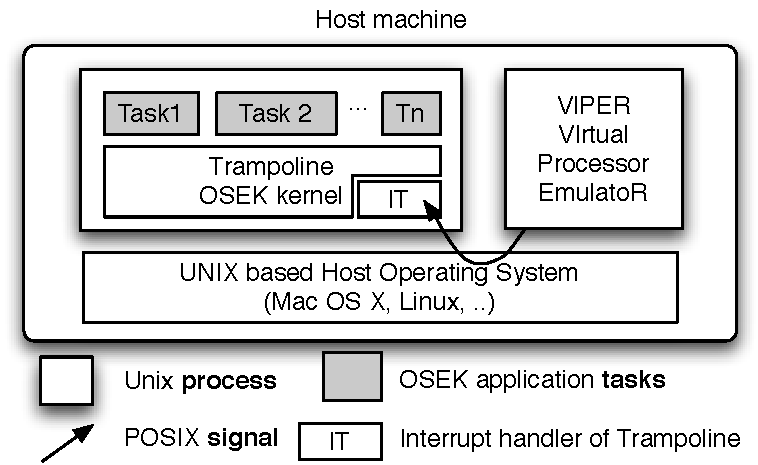
\includegraphics[width=.5\textwidth]{./img/viper.pdf}
\end{center}
\label{fig:viper}
\caption{ViPer}
\end{figure}

TODO

\chapter{Lab 1 -- Understanding fixed priority scheduling}

\section{Goal}

The goal of this lab is to become familiar with the development
process of application using Trampoline RTOS, and to understand how fixed priority scheduling works.
We will also see Events.

Trampoline includes an OIL compiler.
It reads a static description of the objects of the application (tasks,
ISRs, events, resources, etc.) and generates the corresponding OS data structures.
In addition to the OIL description, the developer must of course provide the C
source code of the body of tasks and ISRs.


\section{Starting point}

Go into the lab1 directory. There are 2 files:

\begin{description}
    \item[lab1.oil] a minimal OIL description.
    \item[lab1.cpp] a minimal source code.
\end{description}

Edit the lab1.oil file and update the \texttt{TRAMPOLINE\_BASE\_PATH} attribute
in function of your configuration: it should point to the directory where Trampoline is installed.

lab1 is a very simple application with only 1 task named \texttt{task1}. It
starts automatically (\texttt{AUTOSTART = TRUE \{ ... \}} in the OIL file) and
prints "\texttt{Hello world}" on the terminal.

To compile this application, go into the lab1 directory and type (on a single line):

%\namedtodo[JLB]{update path}
\unixcl{\parbox{\linewidth}{%
goil\blanc{}--target=posix\blanc{}--templates=/opt/trampoline/goil/templates/\blanc{}lab1.oil}}

The \texttt{--target} option is used to define the target system (here we generate the OS level data structures of Trampoline for the \texttt{posix} target).
The \texttt{--templates} option indicates where to find the template files used to generate the configuration of the kernel.

Alongside the C files of the kernel configuration, Goil also generates a build script for the application (files \texttt{make.py} and \texttt{build.py}).

If you change something in the OIL file or in your source code file, you do not need to re-run Goil because the build script should run it when needed.

Continue the build process by typing:

\unixcl{./make.py}

The application and Trampoline OS are compiled and linked together.
The target file is named \texttt{lab1\_exe}.

To run the application, simply run the application:

\unixcl{./lab1_exe}

The program starts and prints the message. As soon as the job of Task1 is terminated, Trampoline gets into idle (starting an internal idle task). To terminate the process, simply type \unixcl{Ctrl+C}.



\section{OS system calls and tasks}

For each question, you should create a copy of the lab1 directory and change its name to \texttt{lab1q1}, \texttt{lab1q2}, \ldots

\subsection{Task activation and scheduling}

The \texttt{ActivateTask()} system call allows to activate a task of the application.

\begin{ex}
    Add two tasks in the system: \texttt{task2} and \texttt{task3}.
    \begin{itemize}
		\item add the declaration of both tasks in the description file (OIL file); \texttt{task2} should have priority 1 and its AUTOSTART attribute should be set to FALSE; \texttt{task3} should have priority 8 and its AUTOSTART attribute should be set to FALSE;
		\item in the implementation file (C file), you should:
            \begin{itemize}
                \item provide the body of each tasks:
                    \begin{itemize}
						\item task \texttt{task2} prints "\texttt{==Task2==}" on the terminal;
                        \item task \texttt{task3} prints "\texttt{==Task3==}" on the terminal;
                    \end{itemize}
                \item and, lastly, modify task \texttt{task1} so that is activates \texttt{task2} and \texttt{task3} (in this order).
            \end{itemize}
    \end{itemize}

	Before to execute the resulting application, draw a schedule and give the text written on the terminal
    Your diagram must clearly show activation, execution and termination of each job using symbols used in the course.
    Then execute the application and check the correctness of your diagram.
\end{ex}

%\subsubsection{Using the debugger to follow the scheduling}
%\namedtodo[SF]{add text on gdb, add \texttt{init.gdb}
%  in code.}{TODO}
%
%\begin{ex}
%  Run the application step by step with the debugger and follow the scheduling.
%  Identify precisely the preemption point in the code of each tasks.
%\end{ex}


\subsubsection{Trace evaluation}
%TODO:
% On parle du READY_AND_NEW qui est un état interne… ici, avant?
%
It is not possible to measure timings on this virtual platform. However, The trace allows an analysis of the behavior after execution (post-mortem). To get the trace (after an execution) on standard output:

\begin{lstlisting}
./readTrace.py
\end{lstlisting}

To redirect the output to a file (\texttt{output.txt} here), simply write the command:
\begin{lstlisting}
./readTrace.py >output.txt
\end{lstlisting}


There is one event per line, beginning with the current date (based on \texttt{SystemCounter} value).

Even if the date is the same for several lines, the events (1 per line) are recorded chronologically in the trace file.

Analyze the trace of the current application run, and report on the gantt diagram each events on tasks states.

\subsection{Task chaining}

The \texttt{ChainTask()} system call allows to chain the execution of a task: the calling job terminates and a new job of the target task is created.

\begin{ex}
	%principe base ChainTask
	Starting from the application of question~1, replace the call to \texttt{ActivateTask(task3)} and \texttt{TerminateTask} by a \texttt{ChainTask(task3)} at the end of task \texttt{task1}.
    Draw a schedule of the new system. Then execute the application to check the correctness of your diagram.
    Comment on the differences with the previous application. Explain the differences with the 2 traces.
\end{ex}

\begin{ex}
	%ACTIVATION=1 => 1 fois
    Chain to \texttt{task2} instead of \texttt{task3}.
    Update task \texttt{task2} so that it prints something each time it is executed.
    Draw a schedule of the new system.
    Then execute the application to check the correctness of your diagram.
    Comment on the differences with the previous application.
\end{ex}

\begin{ex}
	%ACTIVATION
    Test the error code returned by ChainTask.
    Modify the OIL file so that ChainTask returns \texttt{E\_OK}.
    Draw a schedule of the new system.
    Then execute the application to check the correctness of your diagram.
    Comment on the differences with the previous application.
\end{ex}

\begin{ex}
	If we wanted to measure the execution time, of \lstinline{ChainTask}, we would have to use a timer as stopwatch. Explain where it should be started and stopped in the following cases:
    \begin{itemize}
        \item fully preemptive scheduling, activation of a higher priority task.
        \item fully preemptive scheduling, activation of a lower priority task.
        \item fully non preemptive scheduling, activation of a higher priority task.
        \item fully non preemptive scheduling, activation of a lower priority task.
    \end{itemize}

    Explain how to use the timer functions for each case and explain the results.
\end{ex}

\section{Extended tasks and synchronization using events}

\textcolor{red}{\emph{For the following exercises, you should use full preemptive scheduling mode.}}

Unlike a basic task, an extended task may wait for an event.
In terms of scheduling, a job is activated when a task is activated or when it leaves the waiting state.

Before to proceed with the following questions, consult the slides of the course to become familiar with events in Trampoline.

%In the OIL file, set the priority of \texttt{task_0} to 8 and add two events \texttt{evt_0} and \texttt{evt_1}. \texttt{evt_0} is used by \texttt{task_0} and \texttt{evt_1} is used by \texttt{task_1}. \texttt{a_task} activates \texttt{task_0} and \texttt{task_1} then sets \texttt{evt_0} and \texttt{evt_1} and terminates. \texttt{task_0} and \texttt{task_1} wait for their event, clear it and terminate.

\begin{ex}
     Based on the application of Question~1, build an application with the following characteristics:
\begin{itemize}
    \item set priority of \texttt{task2} to 8 (so priorities are 1 for \texttt{task1} and 8 for both \texttt{task2} and \texttt{task3});
    \item add two events, \texttt{evt\_2} and \texttt{evt\_3}:
        \begin{itemize}
            \item \texttt{evt\_2} is set by task \texttt{task1} to task \texttt{task2}.
            \item \texttt{evt\_3} is set by task \texttt{task1} to task \texttt{task3}.
        \end{itemize}
    \item modify the code of the tasks:
        \begin{itemize}
            \item task \texttt{task1} activates \texttt{task2} and \texttt{task3} then sets \texttt{evt\_2} and \texttt{evt\_3} before to terminate.
            \item tasks \texttt{task2} and \texttt{task3} wait for their event, clear it, and terminate.
        \end{itemize}
\end{itemize}

Draw a schedule of the new system.
Then execute the application to check the correctness of your diagram (before to run the application, add outputs in the code of the task, for instance writes to the LCD or LEDs to ease the correctness checking).

\end{ex}

\begin{ex}
    Build an application to measure the execution time of \texttt{SetEvent} in the following cases:
    \begin{itemize}
        \item fully preemptive scheduling, setting an event to a higher priority tasks that is not waiting for the event.
        \item fully preemptive scheduling, setting an event to a higher priority tasks that is waiting for the event.
        \item fully preemptive scheduling, setting an event to a lower priority tasks that is not waiting for the event.
        \item fully preemptive scheduling, setting an event to a lower priority tasks that is waiting for the event.
    \end{itemize}

    Explain how to use the timer functions for each case and explain the results.
\end{ex}

\begin{ex}
Program an application conforming to the following requirements:

\begin{itemize}
    \item it is composed of two tasks: \texttt{server} priority 2, \texttt{t1} priority 1.
    \item \texttt{server} is an infinite loop that activates \texttt{t1} and waits for event \texttt{evt\_1}.
    \item \texttt{t1} prints ``I am t1'' and sets \texttt{evt\_1} of \texttt{server}.
\end{itemize}

Before to run the application, draw a schedule of the execution. Add outputs in the bodies of the task (for instance writes to the LCD or the LEDs) to verify your schedule.
\end{ex}

\begin{ex}
Extend the previous application by adding 2 tasks: \texttt{t2} and \texttt{t3} (priority 1 for both) and 2 events \texttt{evt\_2} and \texttt{evt\_3}. \texttt{server} activates \texttt{t1}, \texttt{t2} and \texttt{t3} and waits for one of the events. When one of the events is set, \texttt{server} activates the corresponding task again.

Before to run the application, draw a schedule of the execution. Add outputs in the bodies of the task (for instance writes to the LCD or the LEDs) to verify your schedule.
\end{ex}

%================================================================
\chapter{Lab 2 -- Periodic tasks and Alarms}

\section{Goal}

Real-Time systems are reactive systems which have to do processing as a result of events. You have seen in Lab \#1 how to start processing as a result of an internal event of the system: by activating a task (\texttt{ActivateTask} and \texttt{ChainTask} services) or by setting an event (\texttt{SetEvent} service). In this lab, you will trigger processing as a result of time elapsing (expiration of an Alarm). This lab uses the following concepts: alarm and counter. On the lab board, the Systick timer is used as interrupt source for alarms. The interrupt is sent every 1ms.

\section{First application}

This application implements a periodic task that reads switch button B0 of the board every 100ms.
When switch B0 is open, A3 is turned off.
When button B0 is closed, A3 is turned on.

\begin{ex}
    The \texttt{updateStateOfB0} function implements a small state machine to convert the state of the switch button to states and events.
    Draw this state machine.
    Draw a schedule of the application (the execution of the interrupt service routine associated with the Systick will not be represented; it will be assumed to be negligible).
    Your diagram should show the instants where the state of the switch changes as well as the state of A3.
    Build and execute the application to verify your diagram.
\end{ex}

Modify the application: when B0 is closed, a processing is triggered.
This processing is performed by activating a job of task \texttt{t_process} (priority 3) that, on odd executions, turns on LEDS A4 to A8 and on even executions turns them off.
\begin{ex}
Draw a schedule of the application.
Your diagram should show the physical state of the switch as well as the state of the LEDs (associate numbers with the different state and use these numbers in your diagram).
Build and execute the application to verify your diagram.
\end{ex}


\section{Second application}

The second application will use 2 periodic tasks: \texttt{t1} (priority 2, period 1s) and \texttt{t2} (priority 1, period 1.5s). t1 toggles LED A3 each time it executes and t2 toggles LED A4.

\begin{ex}
    Draw a schedule of the application that show the 20 first states of the LEDs.
    What is the global period of the system?
\end{ex}

The application needs a counter and 2 alarms. Program, build, and run the application.

\section{Third application}

In the third application, alarms, counters, and polling of the switch buttons are mixed.
This application is a system with 2 switches.
After startup, the system is waiting.
When the first switch is closed, the system starts a {\it function}\footnote{Here we mean a function of the application, not a function of the C language.} F that is implemented using a periodic task (period = 1s).
To ``see'' F, uses a blinking LED.
When the first switch is opened, function F is stopped.
When the second switch is closed, the system is shutdown as quickly as possible (ie ShutdownOS\footnote{The ShutdownOS service shutdowns the operating system. All tasks and alarms are stopped. ShutdownOS takes a StatusType argument to specify the kind or error which occurred. In our case use E\_OK as argument.} is called).

\begin{ex}
    Explain the design of the application: provide the list and configuration of tasks and alarms.
    Draw schedules showing different executions.
    Build and execute the application to verify your diagrams.
\end{ex}

Requirements change. Now function F implementation needs an Init code
(runs once when F is started) and a Final code (runs once when F is stopped) as shown in the following diagram:

\begin{center}
    \resizebox{14cm}{!}{%
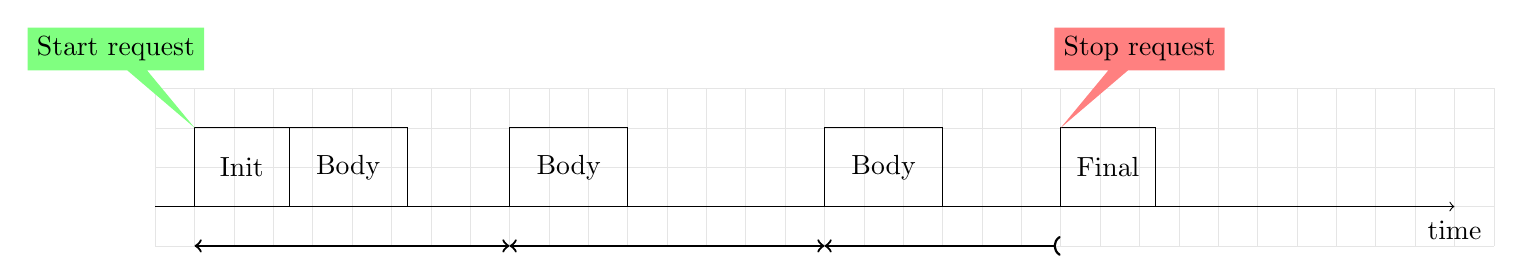
\begin{tikzpicture}
\draw[step=.5cm,gray!20,very thin] (-0.5, -0.5) grid (16.5,1.5);
\draw [->] (-0.5,0) -- (16,0);
\node [yshift=-3mm] at (16,0) {time};
\draw (0,0) rectangle (1.2,1);
\node at (0.6,0.5) {Init};
\draw (1.2,0) rectangle (2.7,1);
\node at (1.95,0.5) {Body};
\draw (4,0) rectangle (5.5,1);
\node at (4.75,0.5) {Body};
\draw (8,0) rectangle (9.5,1);
\node at (8.75,0.5) {Body};
\foreach \x in {0, 4}
  \draw [xshift=\x cm,thick,<->] (0,-0.5) -- (4,-0.5);
\draw [xshift=8 cm,thick,<-(] (0,-0.5) -- (3,-0.5);
\draw [xshift=11cm] (0,0) rectangle (1.2,1);
\node [xshift=11cm] at (0.6,0.5) {Final};
\node [rectangle callout, fill=green!50, callout absolute pointer={(0,1)}] at (-1,2) {Start request};
\node [rectangle callout, fill=red!50, callout absolute pointer={(11,1)}] at (12,2) {Stop request};
\end{tikzpicture}
} %% resizebox
\end{center}


\begin{ex}
    Modify the application to take the new requirements into account.
    Your implementation will use only basic tasks.
    Each phase of F (Init, Body, and Final) is executed in a different task.
    Explain the design of the application: provide the list and configuration of tasks and alarms.
    Draw schedules showing different execution scenarii.
    Build and execute the application to verify your diagrams.
\end{ex}

\begin{ex}
    Same question as above, but your implementation will use an extended task to control the execution of Init, F, and Stop.
\end{ex}

\section{Fourth application}

In this part, you will implement a watchdog. It is a mechanism that allows to stop a processing or a waiting period once a delay has elapsed.

In your application, each time B0 is closed, B3 must be pressed within 4 seconds. In this case, you print the time between the two occurrences. Otherwise, an error message is displayed. If B0 is closed more than once are within 5 seconds from the first time, these events are ignored.

\begin{ex}
    Specify this behaviour with a state machine.
    What is happening if the timeout occurs just after B3 has been closed but before the waiting task got the event?
    Design and program a solution that handles this situation correctly.
    Draw a schedule of the behaviour of your application in such a scenario (this schedule should show the state of the alarms).
\end{ex}

\section{Fifth application}

Program a chase\footnote{chenillard in French} with a 0.5s period. To do so, use 8 periodic tasks. Each periodic task manages a LED. The chase effect is done by using alarms with a time shift between them.

When B0 is closed, the chase starts, when it is opened, it is reset.
When B3 is closed, the chase stops until B3 is opened.
When B2 is closed, the chase direction changes (even if it is stopped).

\begin{ex}
    Specify the high level behaviour with a state machine.
    Design and program the application.
    Explain your design.
\end{ex}

%%================================================================
\chapter{Lab 3 -- Shared object access protection}

To show resources usage, we will use a bad program that allows to corrupt a shared global variable which is not protected against concurrent writes. This has been presented in the course. This lab will show different ways to prevent this wrong behavior by using resources (standard and internal) or other solutions (preemption and priority).

To ensure that the compiler does not hide our bug, update the value of the \texttt{CFLAGS} key in the OIL file: replace option \texttt{-Os} by \texttt{-O0} to turn off all optimizations.

\section{Application requirements}

The diagram of figure~\ref{fig:appdiag} describes the application.
It is composed of 3 tasks that share 2 global variables {\bf declared with the volatile keyword}: \texttt{val} and \texttt{activationCount}:
\begin{itemize}
\item a background task called \texttt{bgTask}, activated at startup. In an infinite loop it increments then decrements the global variable \texttt{val}. This task has priority 1.
\item a periodic task called \texttt{periodicTask} that activates a job every 50ms. This periodic task increments the global variable \texttt{activationCount}. If \texttt{activationCount} is odd, \texttt{val} is incremented, otherwise it is decremented. This task has priority 10.
\item a periodic task \texttt{displayTask} that runs every 2 second and prints \texttt{val} on the LCD. This task has priority 2.
\end{itemize}

\def\alarm#1#2{
  \node[alarm](#1) [#2] {};
  \coordinate (a) at ($(#1.north)$);
  \coordinate (b) at ($(#1.north east)$);
  \coordinate (c) at ($(#1.north west)$);
  \coordinate (d) at ($(#1)$);
  \draw[thick] ($(a)+(-0.1,0)$) rectangle ($(a)+(0.1,0.1)$);
  \draw[rotate=-45,thick] ($(b)+(-0.05,0)$) rectangle ($(b)+(0.05,0.1)$);
  \draw[rotate=45,thick] ($(c)+(-0.05,0)$) rectangle ($(c)+(0.05,0.1)$);
  \draw ($(d)+(0.3,0)$) -- (d) -- ($(d)+(0,0.3)$);
  \node [font=\scriptsize,below=0.5mm of #1] {{\em Alarm}}
}

\def\sharedvar#1#2#3{
  \node (#1) [#2] {#1};
  \coordinate (a) at ($(#1.north #3) + (0,0.2)$);
  \coordinate (b) at ($(#1.south #3) + (0,-0.2)$);
  \draw[ultra thick] (a) -- (b);
  \draw ($(a)+(-0.1,0)$) -- ($(a)+(0.1,0)$);
  \draw ($(b)+(-0.1,0)$) -- ($(b)+(0.1,0)$)
}

\def\varrect#1{
  \draw ($(#1.south west)$) rectangle ($(#1.north east)$)
}

\begin{figure}[htbp] %  figure placement: here, top, bottom, or page
   \centering
   \begin{tikzpicture}[
   task/.style={draw,very thick,fill=white,drop shadow={opacity=0.25},text width=2.5cm, text centered, minimum height=1.5cm},
   alarm/.style={draw,thick,circle,fill=white,drop shadow={opacity=0.25},text width=.5cm}
   ]
   \node[task](periodicTask) at (0,0) {periodicTask};
   \node[task](bgTask) [above=of periodicTask] {bgTask};
   \node[task](displayTask) [above=of bgTask] {displayTask};
   \alarm{activateDisplay}{left=20mm of displayTask};
   \alarm{activatePeriodic}{left=20mm of periodicTask};
   \sharedvar{val}{left=of bgTask}{east};
   %\sharedvar{activationCount}{right=of periodicTask}{west};
   \sharedvar{stdout}{right=of displayTask}{west};
   \varrect{stdout};
   \draw [thick,<->] (val.east) -- (bgTask.west);
   \draw [thick,->] (val.north east) -- ++(5mm,0) |- ($(displayTask.south west) + (0,2mm)$);
   \draw [thick,<->] (val.south east) -- ++(5mm,0) |- ($(periodicTask.north west) + (0,-2mm)$);

   \draw [thick,->] (activateDisplay.east) -- ++(5mm,0) -- ++(0,1.5mm) -- ++(3mm,-3mm) -- ++ (0mm,1.5mm) -- (displayTask);
   \node at ($(activateDisplay.east) + (6.5mm,-3mm)$) {2s};
   \node[font=\scriptsize] at ($(activateDisplay.east) + (9mm,3mm)$) {{\em ActivateTask}};
   \draw [thick,->] (activatePeriodic.east) -- ++(5mm,0) -- ++(0,1.5mm) -- ++(3mm,-3mm) -- ++ (0mm,1.5mm) -- (periodicTask);
   \node at ($(activatePeriodic.east) + (6.5mm,-3mm)$) {50ms};
   \node[font=\scriptsize] at ($(activatePeriodic.east) + (9mm,3mm)$) {{\em ActivateTask}};
   %\draw [thick,<->] (activationCount.west) -- (periodicTask);
   %\draw [thick,->] (activationCount.north west) -- ++(-5mm,0) |- ($(displayTask.south east) + (0,2mm)$);
   \draw [thick,->] (displayTask) -- (stdout);
   \end{tikzpicture}
   \caption{Application diagram}
   \label{fig:appdiag}
\end{figure}

\begin{ex}
    Before programming the application, gives the expected sequence of values for val.
    Design, program, and run the application.
    Now, decrease gradually the period of task \texttt{periodicTask} and observe the sequence of values of val.
    Comment.
\end{ex}


%Compile again your application but add a \unixcl{CFLAGS = "-O3"} in the OIL file. This flag
%makes the C compiler optimize the assembly code.

%\begin{ex}
%Is it the same behavior as in previous question? Why?
%\end{ex}



\section{Global variable protection}

%Remove the \unixcl{CFLAGS = "-O3"} from the OIL file. As shown in the course, we must protect the access to the global variable.

Update the OIL file and the C program to protect the access to the global variable \texttt{val}. Use a resource to do it.

The resource priority is automatically computed by goil according to the priorities of the tasks which use it.

The OIL compiler generates many files in the directory bearing the same name as the oil file (without the .oil suffix). Among them 3 are of interest for this lab:
\begin{itemize}
\item \texttt{tpl_app_define.h}
\item \texttt{tpl_app_config.h}
\item \texttt{tpl_app_config.c}
\end{itemize}

The file \texttt{tpl_app_config.c} contains the tasks descriptors among other data structures. These structures are commented.

\begin{ex} ~
    \begin{itemize}
        \item
            Recall the computation rule of the ceiling priority of a resource with the immediate ceiling protocol.
            According to this rule, what should be the ceiling priority of the resource?
        \item
            Find the actual ceiling priority in \texttt{tpl_app_config.c}. Is it the expected value? If not, is it a problem?
    \end{itemize}
\end{ex}

%To observe the impact of the priority ceiling protocol, use the following function to observe the priority of the jobs during their execution.

%\begin{lstlisting}[language=C]
%void displayIdAndCurrentPriority()
%{
  %TaskType id;
  %GetTaskID(&id);
  %if (id >= 0)
  %{
    %tpl_priority prio = (tpl_dyn_proc_table[id]->priority) >> PRIORITY_SHIFT;
    %lcd.print("Id=");
    %lcd.print(id);
    %lcd.print(", Prio=");
    %lcd.print(prio);
  %}
%}
%\end{lstlisting}

%And you have to add the following line at start of your C file:

%\begin{lstlisting}[language=C]
 %#include "tpl_os_task_kernel.h"
%\end{lstlisting}


\section{Protection with an internal resource}

An internal resource is automatically taken when the job gets the CPU, and released when it terminates. Replace the standard resource by an internal resource in the OIL file. Remove the \texttt{GetResource} and \texttt{ReleaseResource} in the C file.

\begin{ex}~
    \begin{itemize}
        \item
            What happens? Why?
        \item
            How to solve the problem? Draw a schedule of a correct implementation of the system. Program this solution.
    \end{itemize}
\end{ex}


\section{Protection using a single priority level}

\begin{ex}
Modify the OIL file: remove the resource and set the priorities so that all tasks share the same priority. Draw a schedule of the system.
\end{ex}

\section{Protection using fully non preemptive scheduling mode}

\begin{ex}
Modify the OIL file: all tasks are now non preemptive. Draw a schedule of the system.
\end{ex}

%%%% TODO : mettre à jour la question qui suit. Maintenant que Trampoline est installé dans /opt
%%%% et que les fonctions du TFT et de l'expandeur sont en libs dans machines/, les
%%%% étudiants ne peuvent plus ajouter les ressources dans le code.

\section{Upgrading the coro\_utils function}

\begin{ex}
    As explained in section~\ref{sec:coroutils}, both the screen and the IO
    expander use the SPI interface of the MCU. Thus, to ensure coherency of SPI
    transactions, we have avoided using both devices in the same application.
    However, using resources, it is possible to enforce mutual exclusions
    between concurrent tasks that use the SPI.
    Design and program such an application.
\end{ex}

\chapter{Lab4\\Internal communication}

\section{Overview}

Internal messaging may be used as an easy to use replacement for shared variables. Messaging allows to send data between tasks. This lab will show the different ways to communicate in OSEK.

Design a first simple application with 2 communicating tasks.
The OIL file declare 2 tasks: \texttt{sender} and \texttt{receiver} and 2 messages: \texttt{outMessage} and \texttt{inMessage}. \texttt{inMessage} is connected to \texttt{outMessage}. Task \texttt{sender} uses \texttt{outMessage} and task \texttt{receiver} uses \texttt{inMessage}.

Task \texttt{sender} is activated every second by the mean of an alarm and sends data to \texttt{outMessage}.
Send for instance the number of activation of task \texttt{sender}.
When the data is received in \texttt{inMessage}, the notification mechanism activates task \texttt{receiver}.
\texttt{receiver} reads the data from \texttt{inMessage} and prints the value.

Notice that message identifiers must be declared before to be used in the source file with \texttt{DeclareMessage}.

\section{Message broadcasting}

OSEK messaging supports \emph{many-to-many} communication. This is done by having more than one receiving messages connected to the same sending message.
\begin{ex}
Add 2 other receiving messages connected to \texttt{outMessage}. The first message activates the task \texttt{Emergency} (add the corresponding task), the second message sets an event to task \texttt{NormalOperation} (add the corresponding extended tasks too). Write the C code of the tasks you added. The first one receives the message and prints the value; the second one waits for the event in an infinite loop, receives the message and prints the value. Check the application works as expected.
\end{ex}

\section{Filtering}

\begin{ex}
Add a filter to activate task \texttt{receiver} upon the 4th message and then every 3 values (ie 4th, 7th, 11st and so on).
\end{ex}

\begin{ex}
    Modify task \texttt{sender} to send  pseudo-random values ranging from 0 to 100 (you can use for instance xorshift32 as described here:\url{https://en.wikipedia.org/wiki/Xorshift}) and then a modulus.
    Using filtering, set the event to task \texttt{NormalOperation} only if the value is within the range $[20,60]$; activate task \texttt{Emergency} only if the value is not within the range.
\end{ex}

\section{Queued messages}


\begin{ex}
    Restarting with the Messaging application, modify the \texttt{inMessage} to make it a queued message with a size of 4 data items and remove the notification. Add an alarm to activate task receiver every 4 seconds. Check the return value of \texttt{ReceiveMessage} and verify that no error occurred (queue under- or over-flow). If errors occur, correct the application.
\end{ex}

\end{document}
